\documentclass[12pt]{article}
\usepackage{graphicx} % Required for inserting images
\usepackage{parskip}
\usepackage{float}
\usepackage{multirow}
\usepackage{booktabs}
\usepackage{appendix}

\usepackage[T1]{fontenc}
\usepackage{palatino}

\usepackage[margin=1in]{geometry} % adjust margins

\title{County Level MIPS Quality Scores: Coverage Limits and Association with Medicare Outcomes}
\author{Transaint Gau, Maria Paz, Zachary Sletten, Justin Tseng}
\date{August 18, 2026}

\begin{document}

\maketitle

\section{Abstract}
% Project Statement
Medicare's \textbf{M}erit-based \textbf{I}ncentive \textbf{P}ayment \textbf{S}ystem (MIPS) scores physician groups on quality and adjusts payment \cite{Lin2025Merit-BasedYears}. We test whether county aggregates of those scores help predict Medicare outcomes after accounting for county demographic and specialty characteristics. Using 2023 public data \cite{2023PYAttestations, 2026MedicareCounty, 2023DoctorsFile}, we examine whether counties form clear clusters based on MIPS performance and compare models of all cause hospital readmission within 30 days using county controls alone and with MIPS measures added. Counties did not form distinct groups based on their MIPS scores. Among the 2,458 counties with a published readmission rate, adding MIPS to county controls improved prediction only slightly (Elastic Net $R^2$ +0.017), and a 95\% interval for that gain included zero, meaning it could be no improvement at all. On the 2,444 counties with a 2022 readmission rate, the increment was +0.006 before that rate was included as a control and +0.002 after. 69.2\% of county measure cells were based on two or fewer reporting practices, limiting their value as a regional quality signal. These findings describe county aggregates of publicly reported scores. Assessing effects on care or individual practices would require more granular data and a different study design.

\section{Introduction}

\subsection{Background}
Established by Centers for Medicare \& Medicaid Services, the \textbf{M}erit-based \textbf{I}ncentive \textbf{P}ayment \textbf{S}ystem (MIPS) is a system designed to transition Medicare clinicians towards a value-based care system. It determines clinician performance across four different categories (quality of care, improvement activities, electronic medical record interoperability, and cost) and provides an ultimate score that determines the reimbursement rate for that clinician \cite{Lin2025Merit-BasedYears}. MIPS' effectiveness has been mixed, and as Bond et. al. explain, "The MIPS program may not accurately capture the quality of care that primary care physicians provide" \cite{Bond2022AssociationOutcomes}.

MIPS data is available to the public and freely downloadable \cite{2023PYAttestations}, meaning evaluations of the system's efficacy can be performed. MIPS links reported performance to payment, so it is useful to examine whether higher scores are associated with better patient outcomes. This is especially relevant as MIPS is designed to be a budget-neutral program \cite{Gettel2022TheSystem}, meaning that their reimbursement is affected not only by their performance, but by other physicians' performance as well (one physician's increase in funding is paid for by another's decrease).

Furthermore, Lin et. al. state that "safety-net specialists did not achieve greater cumulative financial rewards due to MIPS's percentage-based adjustment structure, which disadvantages clinicians with smaller billing volumes" \cite{Lin2025Merit-BasedYears}. MIPS financially rewards performance on selected measures, raising the broader question of whether the behaviors it rewards always align with what is best for patients. This project focuses on a narrower question: whether county aggregates of publicly reported MIPS scores add predictive value for county Medicare outcomes.

In order to measure MIPS, we utilized two other data sources. Our second source was a regional database of patient outcomes \cite{2026MedicareCounty}. This data source has multiple methods of measuring patient health outcomes, and provides a way for us to determine if there exists a strong correlation between those outcomes and MIPS scores. Our final source was a database of doctors and physicians enrolled with Medicare \cite{2023DoctorsFile}. This data source (referred to later as the "DAC") acts as the "bridge" between the first two data sources, allowing us to combine all three into one source for analysis.

\subsection{Outcome Evaluation}
% Evaluation Strategy
Success was defined as whether county aggregated MIPS improves out of sample prediction of county Medicare outcomes beyond what county characteristics already explain. The primary outcome is the 2023 county 30 day all cause readmission rate, with standardized Medicare payment per capita as a secondary outcome. Models are scored on states held out from training, and a mean predictor provides the baseline, so the comparison of interest is the change in cross-validated performance when MIPS measures are added to county controls alone. We then tested whether that gain held across those states, and whether it remained if we used reporting instead of scores. We also checked adjacent years and the prior year's readmission rate. Finally, we asked whether any single measures still stood out after a coverage floor and a multiple testing correction.

\section{Methods}
% Methodology
% Technical Depth
All Python work was split between five Jupyter notebook files. Data Collection (Section \ref{meth_collect}) was completed in Notebook 1. Data Sanitization (Section \ref{meth_sanitize}) and Exploratory Data Analysis (Section \ref{meth_eda}) were completed in Notebook 2. Unsupervised Learning (Section \ref{meth_unsup}) was completed in Notebook 3. Supervised Learning (Section \ref{meth_sup}) was completed in Notebooks 4 and 5.

\subsection[Data Collection]{Data Collection \\ \small{Notebook 1}} \label{meth_collect}
In Notebook 1, we loaded and evaluated our 3 files to assess for missingness, basic data structure, column names to ensure we would be able to merge files reliably. We determined there was a significant percentage of physician groups that had more than one zip code and thus needed to devise a strategy to handle. We determined the files were complete when evaluating the features and variables of interest. We confirmed the files contain the data necessary to merge and evaluate group level performance with regional health outcomes. We were able to determine that some performance measures were inverse meaning lower scores are better.

\subsection[Data Sanitization]{Data Sanitization \\ \small{Notebook 2}} \label{meth_sanitize}
In Notebook 2, we loaded our three data sources from Data Collection (Section \ref{meth_collect}). After loading, we adjusted column names and ZIP code values to prepare for joining all three DataFrames into one DataFrame. We used a left join to combine the MIPS and DAC into one DataFrame object. After standardizing ZIP codes and other small adjustments, we used another left join to add the final patient outcomes DataFrame to create the final DataFrame.

After the consecutive left joins, we continued to sanitize our data. We standardized ZIP codes and converted MIPS performance metrics to a numeric scale, and also made further adjustments to accommodate the patient outcome DataFrame being at the county level only. Once sanitization was complete, we eliminated columns that were deemed unnecessary for the next steps of EDA, supervised learning, and unsupervised learning.

\subsection[Exploratory Data Analysis (EDA)]{Exploratory Data Analysis (EDA) \\ \small{Notebook 2}} \label{meth_eda}
As part of our \textbf{E}xploratory \textbf{D}ata \textbf{A}nalysis (EDA), we looked for a correlation between better HbA1c control (a patient metric used to diagnose diabetes) and patient readmission rate (see Figure \ref{fig:hba1c_readmit}).

\begin{figure}[H]
    \centering
    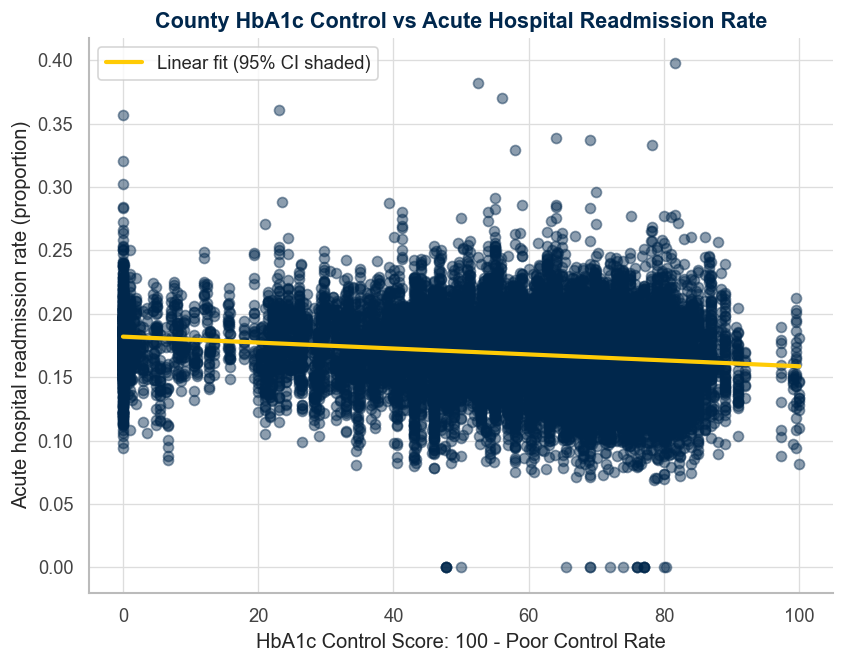
\includegraphics[width=0.95\textwidth]{figures/hba1c_vs_readmission.png}
    \caption{HbA1c vs. Acute Hospital Readmission Rate by county.}
    \label{fig:hba1c_readmit}
\end{figure}


\subsection[Unsupervised Learning]{Unsupervised Learning \\ \small{Notebook 3}} \label{meth_unsup}
For unsupervised learning, we utilized the dataset created in Section \ref{meth_sanitize}. After restricting the available data to rows from 2023, we reshaped the data to one row per county and one column per MIPS measure. Measures reported in fewer than 30\% of counties were removed, followed by counties reporting fewer than 20\% of all 229 measures. This filtering was performed to reduce sparsity and improve the consistency of the data used for clustering. Missing values in the retained matrix were then median imputed, and all measures were standardized prior to dimensionality reduction and clustering.

To determine how many dimensions were needed to represent county MIPS performance profiles, we performed Principal Component Analysis (PCA). We retained the minimum number of principal components required to explain at least 90\% of cumulative variance. Using these retained components, we calculated silhouette scores for K-means clustering with values of $k$ ranging from 2 through 10. We selected the value of $k$ with the highest silhouette score and applied K-means clustering using that value. We then compared Medicare geographic outcomes across the resulting MIPS derived clusters using Kruskal Wallis tests.

\subsection[Supervised Learning]{Supervised Learning \\ \small{Notebooks 4 \& 5}} \label{meth_sup}
For supervised learning we used the 2023 county table from Section \ref{meth_sanitize}. First, we dropped measures reported in fewer than 30\% of counties, leaving 55. Then we dropped counties that reported fewer than 20\% of those 55, leaving 2,507 counties. Clustering used the same 30\% measure rule, but required counties to report 20\% of all 229 measures, which kept only 1,400. The 55-measure county rule includes more counties and needs more imputation. Readmission models use the 2,458 of these counties that have a published readmission rate.

After coverage filtering, we applied three data leakage guards: circular measures, sibling strata, and identity features. First, circular measures are those whose construction overlaps with admissions, readmissions, or complications and therefore shares arithmetic with the outcome. Second, sibling strata are near duplicate versions of the same construct, which would otherwise let one clinical concept enter the model several times. Third, identity features are geographic keys such as state and county FIPS; state defines the cross-validation folds but is excluded from the feature matrix so the model cannot learn a region directly. Of the 55 measures clearing the coverage filter, this screen removes six, leaving 49.

With the feature set settled, six measures are flagged in the source as inverse, where a higher raw value means worse performance. Their coefficients are sign adjusted at display time so that all results are expressed per one standard deviation of better performance. The county controls are beneficiary average age, percent female, percent white, percent Black, percent Hispanic, percent dual eligible for Medicaid, Medicare Advantage participation rate, and log beneficiary count, plus the primary care and advanced practice share of local providers and an indicator marking counties whose race shares are suppressed in the source. The MIPS increment is measured separately as the difference in cross-validated $R^2$ between models fitted with these county controls alone and with controls plus the 49 MIPS measures. We trained multiple supervised learning models on our data (LinearRegression, ElasticNetCV, RandomForestRegressor, and GradientBoostingRegressor) and used GroupKFold with \texttt{state} as our grouping variable to validate the models we trained. Finally, we compared the performance of different combinations of model, features, and targets to select the optimal combination.


\section{Results}

\subsection[Unsupervised Learning]{Unsupervised Learning \\ \small{Notebook 3}}
Of the 229 available MIPS measures, 55 had coverage in at least 30\% of counties. After applying the county coverage threshold, 1,400 of 2,955 counties reported at least 20\% of the retained measures and remained in the clustering dataset. Figure \ref{fig:meas_count} shows that coverage was uneven across both measures and counties, with substantial numbers falling below the selected thresholds.

\begin{figure}[H]
    \centering
    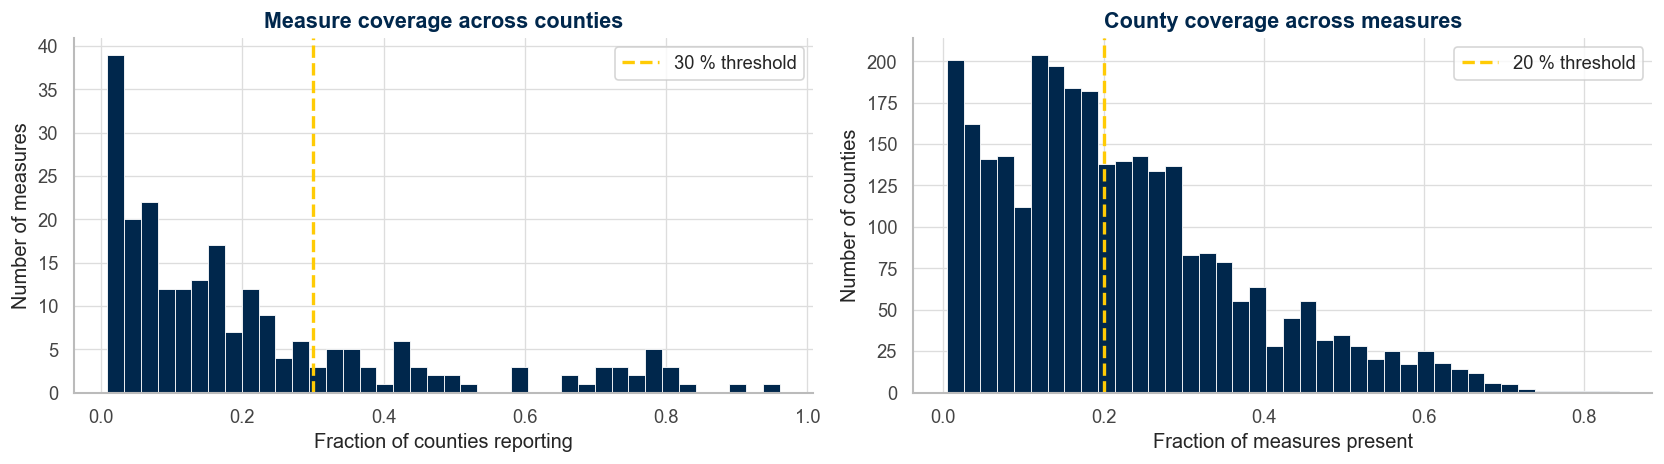
\includegraphics[width=0.95\textwidth]{figures/measure_county_coverage.png}
    \caption{Measure coverage across counties and county coverage across measures.}
    \label{fig:meas_count}
\end{figure}

PCA showed that 41 principal components were required to explain at least 90\% of the cumulative variance across the 55 retained measures. Using these 41 components, the highest silhouette score across $2 \leq k \leq 10$ was 0.096 at $k = 2$. The resulting K-means solution contained two imbalanced clusters consisting of 445 and 955 counties.

Despite the weak separation between clusters, 28 of 44 Medicare geographic outcomes differed between the two clusters at an unadjusted significance threshold of ($p < 0.05$) using Kruskal Wallis tests. The strongest differences involved utilization and cost measures, including standardized payments for tests, home health payments, durable medical equipment costs, and FQHC/RHC visits. Acute outcomes such as hospital readmission and emergency room utilization showed weaker separation between clusters.

\subsection[Supervised Learning]{Supervised Learning \\ \small{Notebooks 4 \& 5}}
We evaluated two targets (Readmission percentage and standardized cost per capita), four models (Linear OLS, Elastic Net, Random Forest, and Gradient Boosting), and two features (control features only and control features with MIPS). Combined with a baseline evaluation, this created 18 total combinations, whose results can be found in Table \ref{tab:model_perf}. 

\begin{table}[H]
\centering
\begin{tabular}{llrrrr}
\toprule
Target & Model & Features & $R^2$ (mean) & $R^2$ (sd) & MAE \\
\midrule
\multirow{9}{*}{Readmission \%}
 & Baseline (mean)   & Ctrl only      & -0.034 & 0.049 & 0.0217 \\
 & Linear (OLS)      & Ctrl only      &  0.126 & 0.053 & 0.0197 \\
 & Elastic Net       & Ctrl only      &  0.130 & 0.050 & 0.0197 \\
 & Random Forest     & Ctrl only      &  0.143 & 0.083 & 0.0193 \\
 & Gradient Boosting & Ctrl only      &  0.082 & 0.095 & 0.0200 \\
 & Linear (OLS)      & Ctrl + MIPS    &  0.117 & 0.066 & 0.0196 \\
 & Elastic Net       & Ctrl + MIPS    &  0.147 & 0.047 & 0.0193 \\
 & Random Forest     & Ctrl + MIPS    &  0.157 & 0.074 & 0.0191 \\
 & Gradient Boosting & Ctrl + MIPS    &  0.102 & 0.081 & 0.0197 \\
\midrule
\multirow{9}{*}{Std. cost per capita}
 & Baseline (mean)   & Ctrl only      & -0.105 & 0.123 & 1321.81 \\
 & Linear (OLS)      & Ctrl only      &  0.027 & 0.289 & 1246.68 \\
 & Elastic Net       & Ctrl only      &  0.031 & 0.264 & 1244.63 \\
 & Random Forest     & Ctrl only      &  0.147 & 0.229 & 1163.34 \\
 & Gradient Boosting & Ctrl only      &  0.100 & 0.224 & 1184.42 \\
 & Linear (OLS)      & Ctrl + MIPS    & -0.010 & 0.282 & 1274.08 \\
 & Elastic Net       & Ctrl + MIPS    &  0.059 & 0.270 & 1230.13 \\
 & Random Forest     & Ctrl + MIPS    &  0.178 & 0.207 & 1145.74 \\
 & Gradient Boosting & Ctrl + MIPS    &  0.162 & 0.227 & 1151.50 \\
\bottomrule
\end{tabular}
\caption{Cross-validated model performance by target and feature set.}
\label{tab:model_perf}
\end{table}

Coverage across the 49 retained measures is thin. Half of all county measure cells rest on a single reporting practice (52.0\%), and 69.2\% rest on two or fewer, so a county's score on a given measure is often one practice's number standing in for the whole county.

We found that Elastic Net was the model that most consistently increased $R^2$ values before and after considering MIPS (see Figure \ref{fig:r2}). 

\begin{figure}[H]
    \centering
    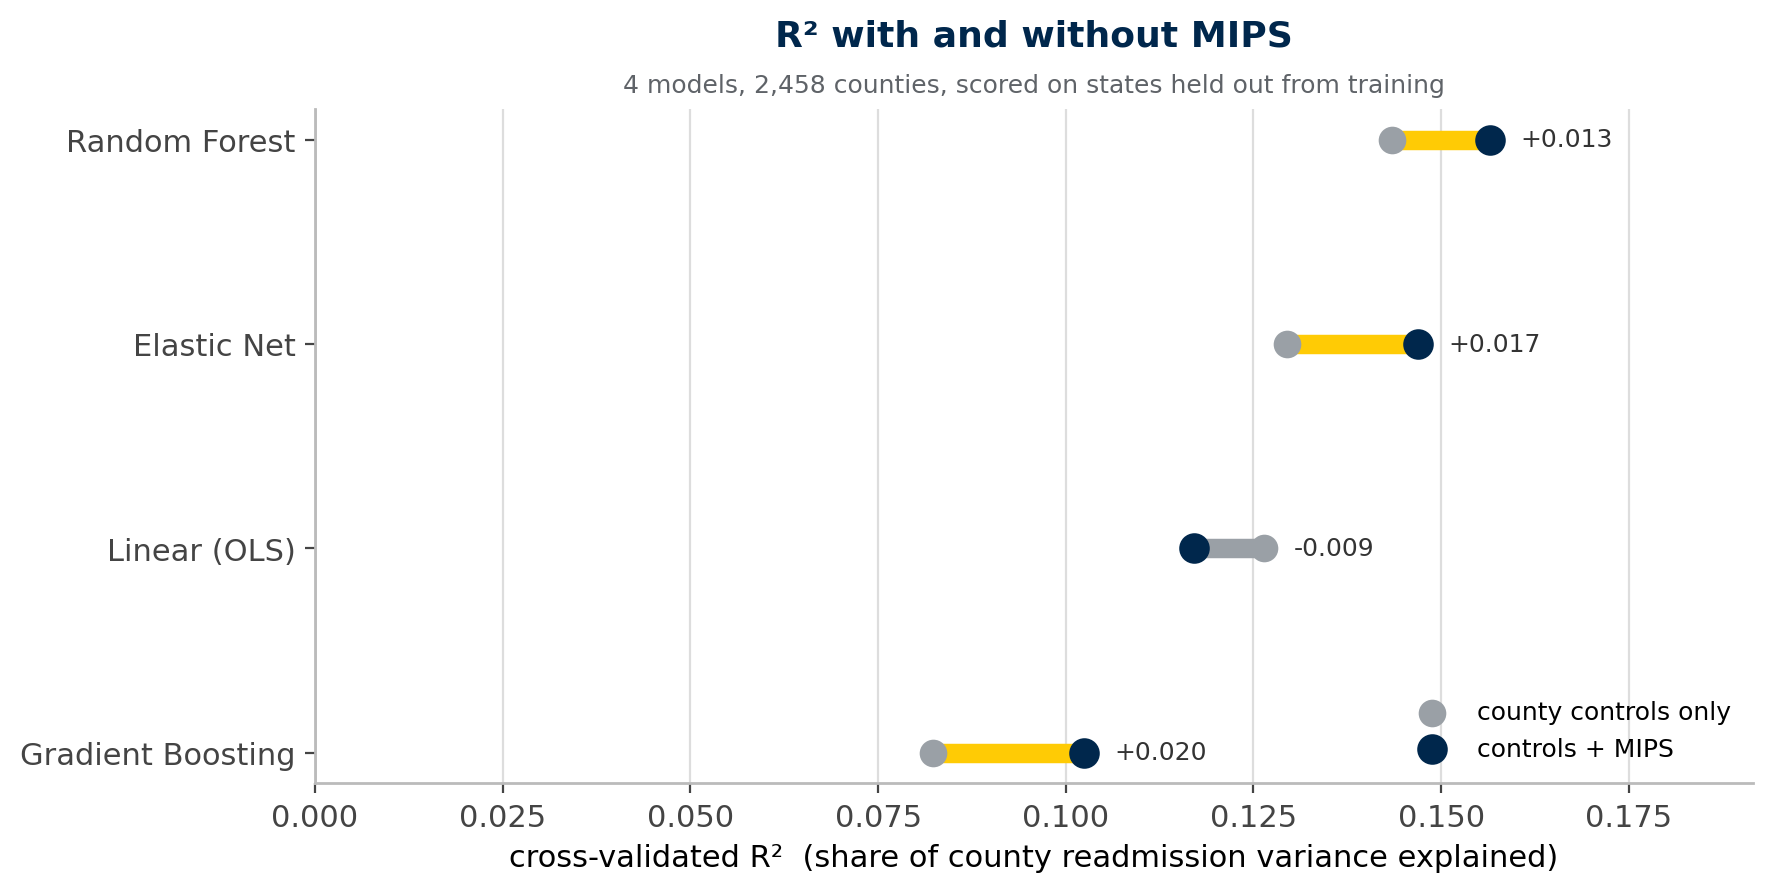
\includegraphics[width=0.95\textwidth]{figures/sl_delta_r2.png}
    \caption{$R^2$ values with and without MIPS.}
    \label{fig:r2}
\end{figure}

The Elastic Net MIPS increment is +0.017 $R^2$, with a 95\% confidence interval of approximately [-0.000, +0.035] (paired $t(4) = 2.78, p = .050$). We quote Elastic Net rather than the largest gain because its increment is positive in all five held out folds; gradient boosting gains more (+0.020) but in only two of five.

Replacing the MIPS values with indicators recording only whether a county reported each measure recovered 81.6\% of the gradient boosting gain (controls .082 $R^2$, reporting indicators .099, actual values .102), suggesting that reporting patterns may account for much of the added signal in that model.

The association is stronger backwards in time. Using the same 2023 MIPS data against outcomes from adjacent years gives MIPS increments of +.043 for 2022, +.020 for 2023, and +.019 for 2024. Since 2023 performance cannot affect 2022 readmissions, this pattern points more toward persistent county characteristics than an effect of MIPS.

Outcome history absorbs the increment. On the 2,444 counties with a prior year readmission rate, MIPS alone adds +.006 $R^2$ while the prior year rate alone adds +.227. With both in the model, the MIPS increment falls to +.002.

A 70\% county-coverage floor leaves 16 of 49 measures eligible for individual testing. Three survive Benjamini-Hochberg (BH) correction: HbA1c poor control (Q001, -0.0029, $q = .007$), cervical cancer screening (Q309, -0.0023, $q = .007$), and breast cancer screening (Q112, -0.0022, $q = .037$). All point in the same direction, with better county performance associated with fewer readmissions.

\begin{figure}[H]
    \centering
    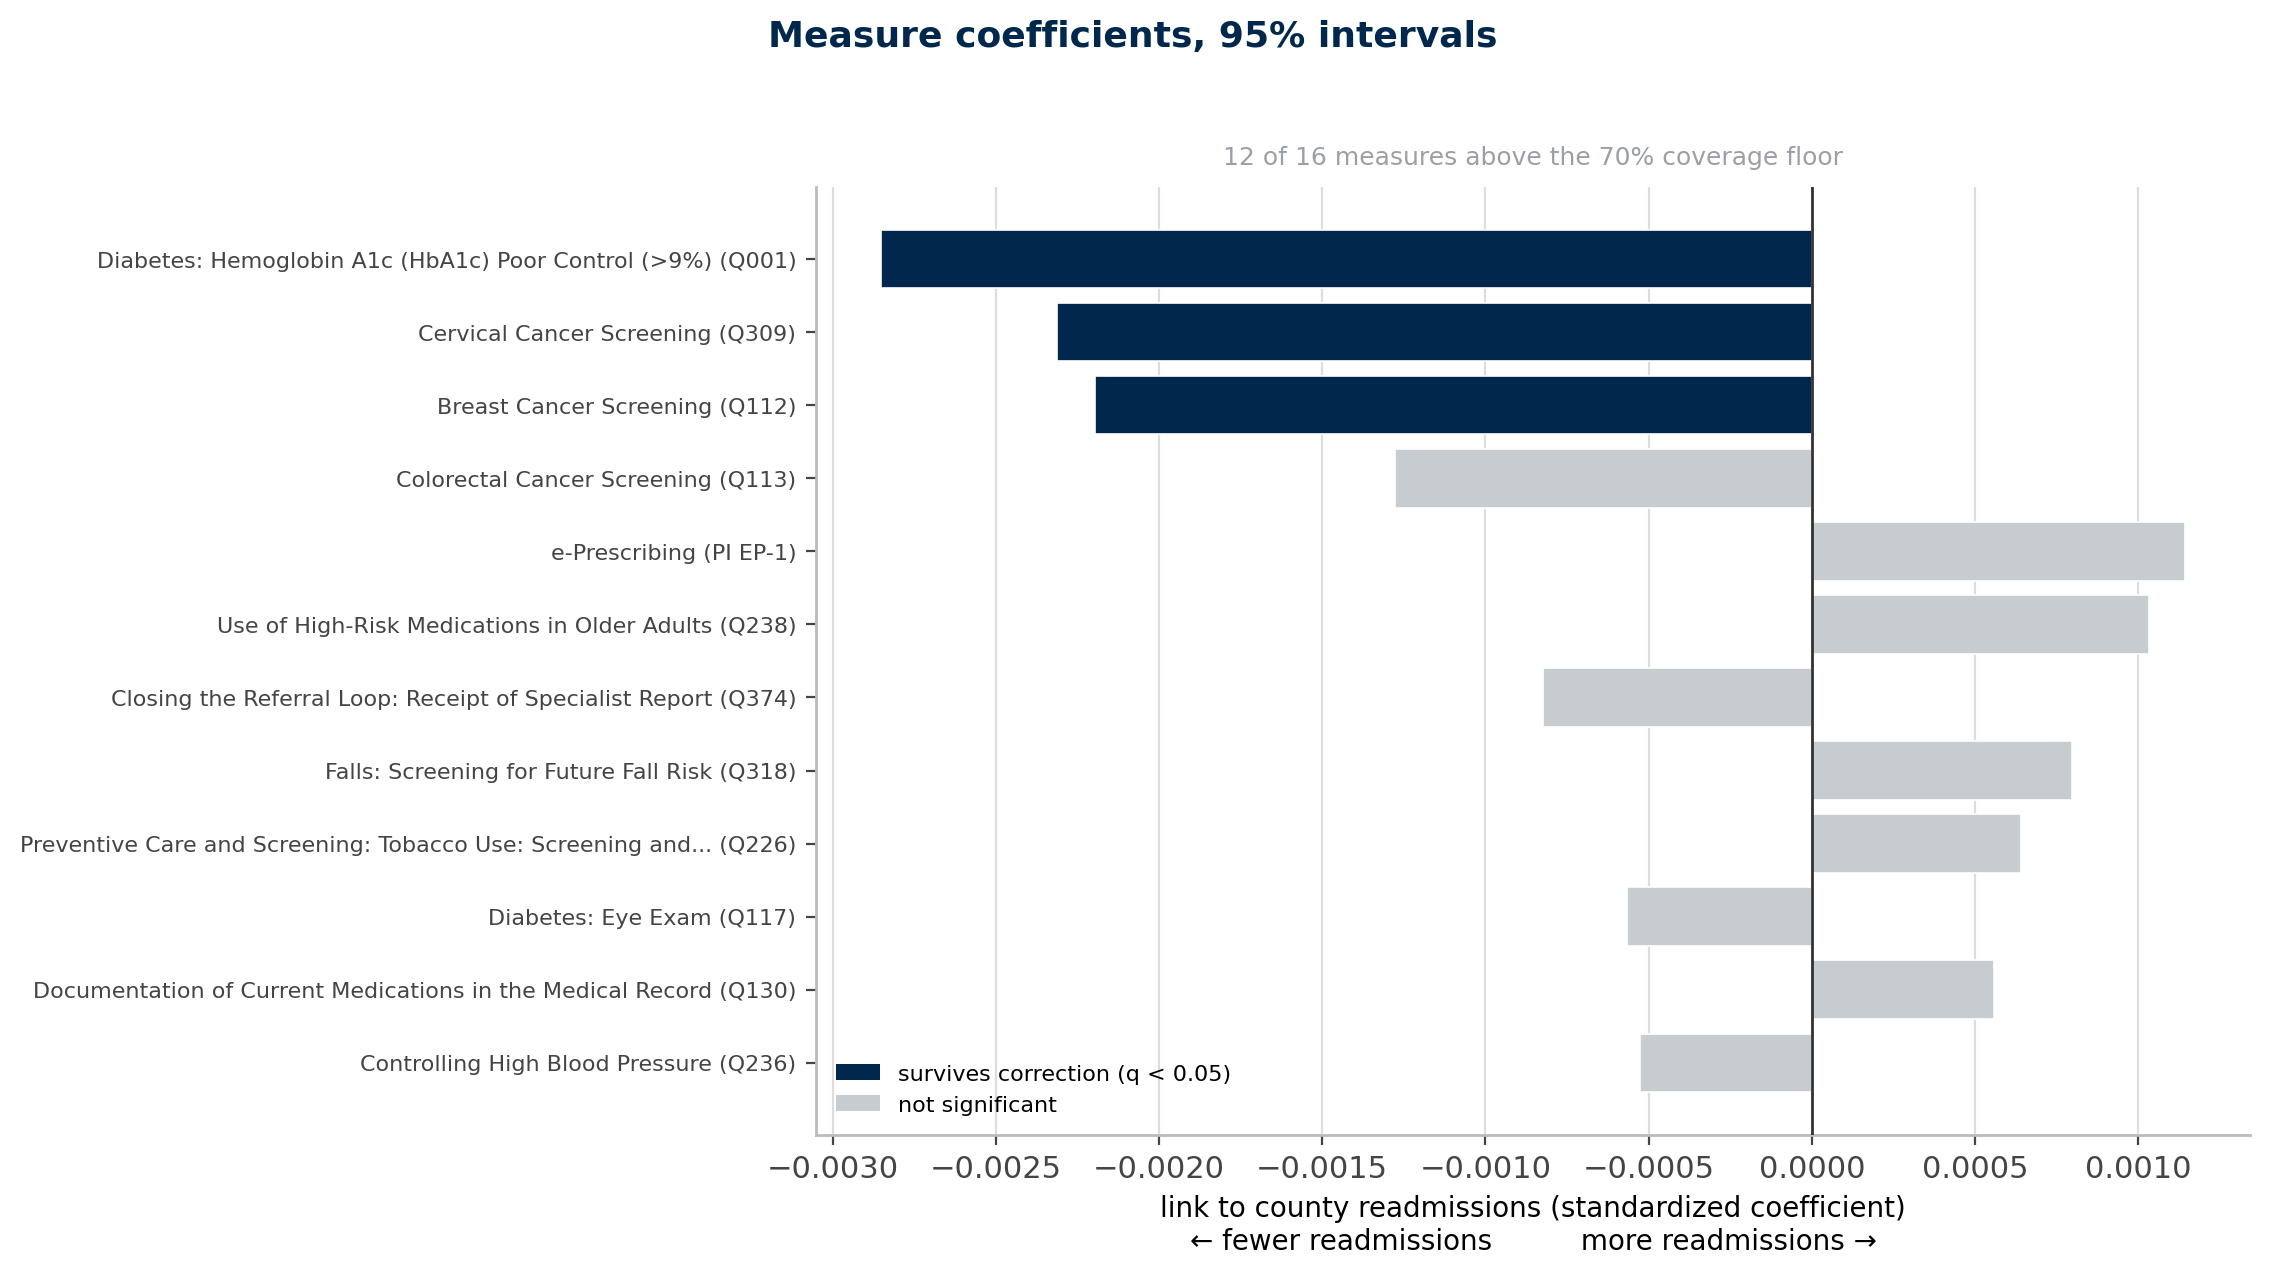
\includegraphics[width=0.95\textwidth]{figures/sl_top_measures_ci.png}
    \caption{The 12 largest of the 16 measures clearing the 70\% coverage floor, with 95\% intervals. Blue indicates the three measures that survive BH correction.}
    \label{fig:ci}
\end{figure}

Model residuals are spatially autocorrelated (Moran's I = +0.199, permutation $p = .001$). All three measures still clear correction under Conley spatial HAC standard errors. Under census division clustering, which uses only nine clusters and is correspondingly conservative, one remains significant.

\begin{figure}[H]
    \centering
    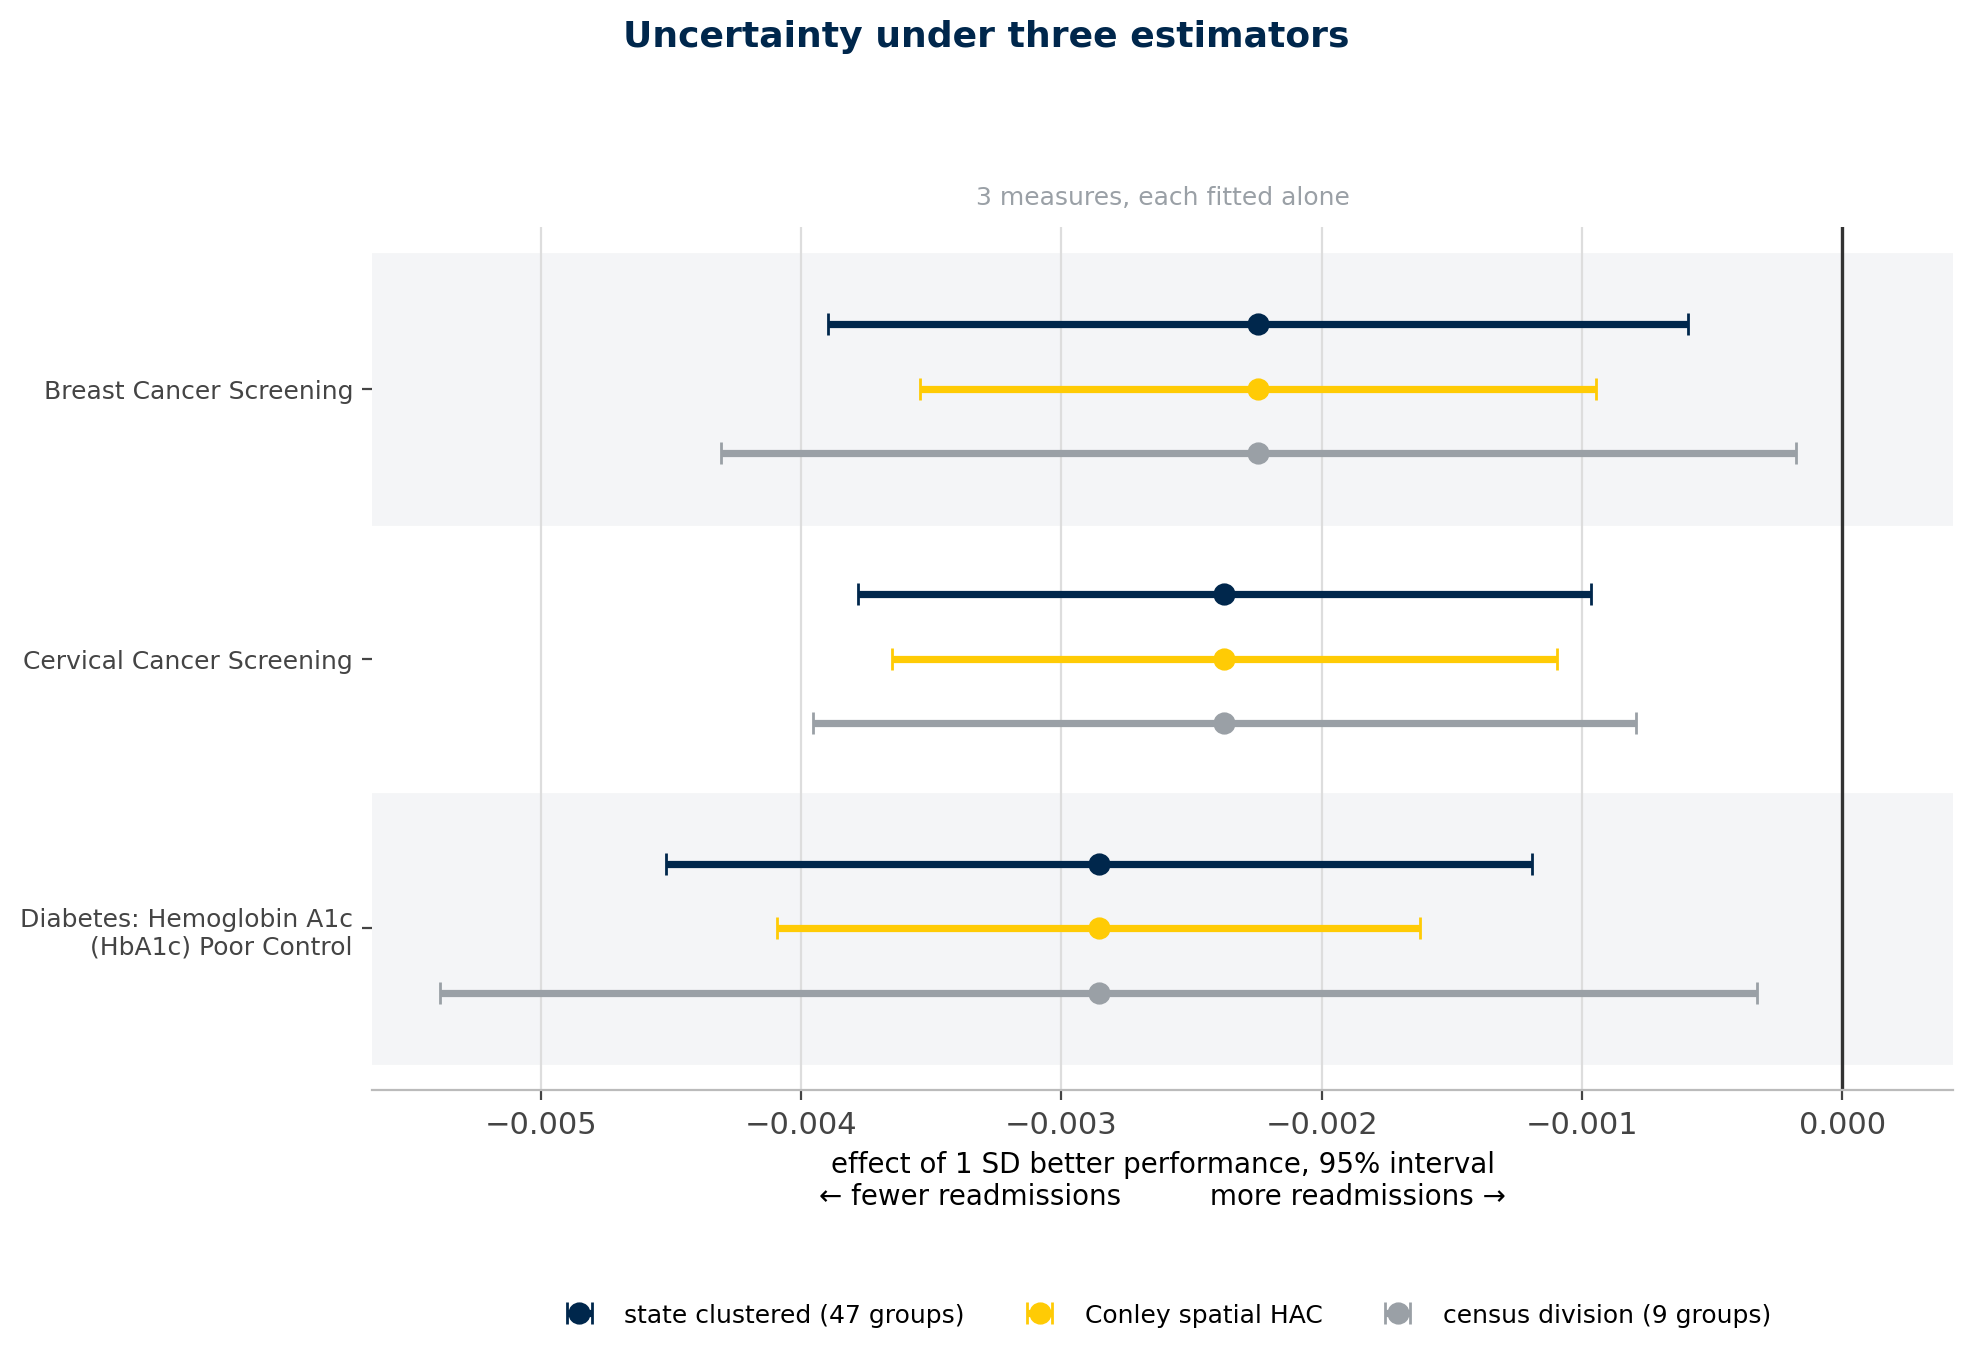
\includegraphics[width=0.95\textwidth]{figures/sl_spatial_forest.png}
    \caption{The three surviving measures under three approaches to estimating uncertainty: state clustered standard errors, Conley spatial HAC, and census division clustering.}
    \label{fig:spatial_forest}
\end{figure}

\section{Discussion}
% Translation
\subsection[Unsupervised Learning]{Unsupervised Learning \\ \small{Notebook 3}}
Our PCA results showed that 41 principal components were required to explain 90\% of the variance across the 55 retained MIPS measures. This indicates that variation in county MIPS performance profiles is distributed across many dimensions rather than being concentrated in one or two dominant components. Consequently, MIPS performance profiles cannot be adequately characterized using only a small number of dimensions.

The best K-means solution occurred at $k = 2$, but its silhouette score of 0.096 was low. This indicates substantial overlap between the two clusters and suggests that counties do not form clearly separated MIPS performance archetypes. The clusters were also imbalanced, with 445 counties in one cluster and 955 in the other. Taken together with the PCA findings, these results suggest that county MIPS performance varies more along a multidimensional continuum than as a small number of clearly separable groups.

Despite the weak cluster separation, 28 of 44 Medicare geographic outcomes differed between the two MIPS derived clusters at an unadjusted $p < 0.05$ threshold. The strongest differences were observed in utilization and cost measures, including standardized payments for tests, home health payments, durable medical equipment costs, and FQHC/RHC visits. In contrast, acute clinical outcomes such as readmission and emergency room utilization showed weaker separation. These findings suggest that differences in county MIPS performance profiles are more closely associated with practice patterns and resource utilization than with patient level acute clinical events.

Several limitations should be considered when interpreting these findings. Approximately 53\% of counties with MIPS data were excluded because they did not meet the minimum coverage threshold, meaning that the clustering results apply only to counties with sufficiently complete MIPS reporting. In addition, median imputation was required for approximately 20\% of values in the retained county by measure matrix, which may reduce true differences between counties. Finally, the analysis is observational and cross sectional, using 2023 MIPS data and 2023 geographic outcomes, so the observed differences between clusters should be interpreted as associations rather than evidence of causal relationships.

\subsection[Supervised Learning]{Supervised Learning \\ \small{Notebooks 4 \& 5}}
County aggregated MIPS appears to be too thin to carry a reliable regional quality signal. With half of county measure cells resting on a single practice, a county's reporting pattern carries nearly as much information as its scores.

The stronger association with 2022 outcomes than with 2024 outcomes suggests that the observed signal may reflect persistent county characteristics rather than a forward effect of 2023 MIPS performance. Prediction residuals remain spatially clustered as well, which is what we would expect if regional factors outside the model drive much of the variation.

These are county level associations and they say nothing about MIPS at the individual practice level where the program operates. Practices are weighted by ZIP-to-county allocation rather than patient volume. Coverage filtering retains counties with more complete reporting, which may affect how representative the analyzed counties are.

\begin{figure}[H]
    \centering
    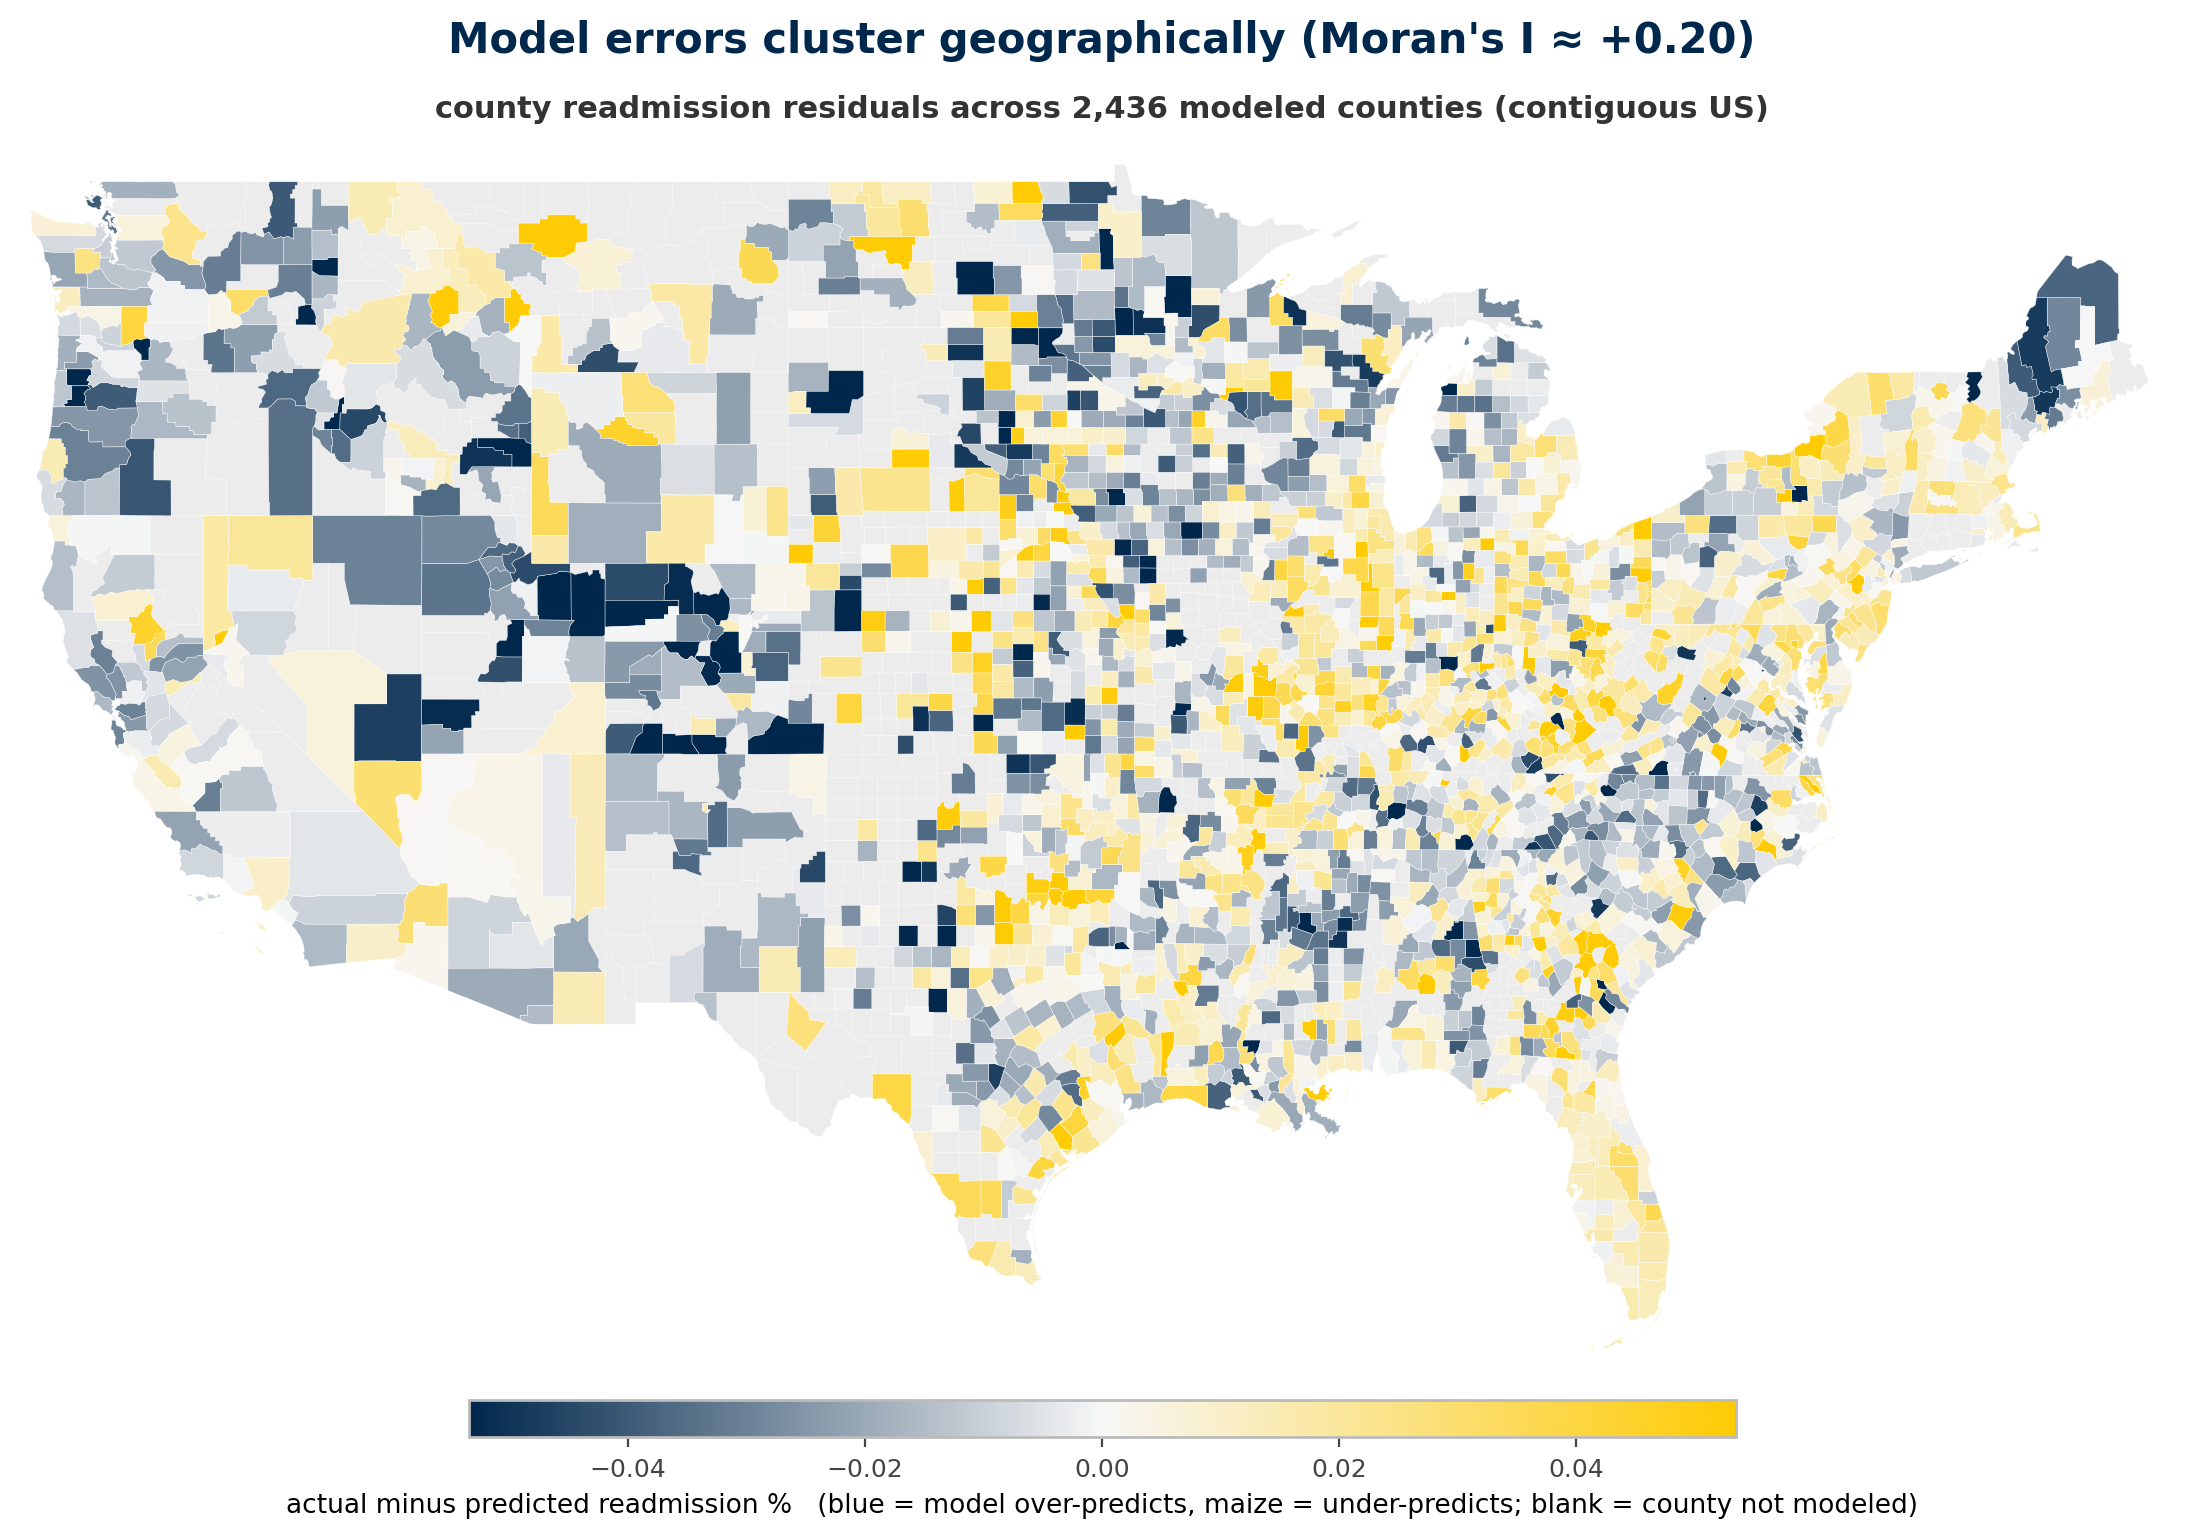
\includegraphics[width=0.95\textwidth]{figures/sl_residual_choropleth.png}
    \caption{Prediction residuals based on county.}
    \label{fig:choropleth}
\end{figure}

\subsection{Broader Impacts}
Ultimately, based on the public data analyzed in this project, county aggregated MIPS scores showed only a weak relationship with Medicare outcomes. This may reflect limits in the available public data and county aggregation, limits in how MIPS measures and rewards quality, or both. Prior research has also found inconsistent links between MIPS scores and patient outcomes \cite{Bond2022AssociationOutcomes} and raised concerns that scores may reflect measure choice and reporting capacity \cite{Apathy2020HighSystem}. Many county values are based on one or two reporting practices, so they may not represent county quality and should not be used to judge an individual practice or physician.

\section{Future Work}
While county aggregated MIPS added little to prediction beyond county controls, there are still opportunities for future work. We could re-run our analysis with different county and measure cutoffs to see if the effects are similar. Another potential path for future work is more granular analysis (i.e., closer than the county level). Counties do not account for population density, so finding a more granular way to compare population centers could yield different results as well.

Another area of future work is comparing MIPS to the reporting system that preceded it. Repeating this county level analysis on earlier public files would not measure how motivated physicians are, but it could show whether the association between reported quality scores and county outcomes was stronger or weaker before MIPS. Since the pre MIPS programs used a different measure set, such a comparison would need measures that are defined consistently across both periods.


\appendix

\newpage

\section{Statement of Work}
% Statement of Work
Each team member contributed equally to the overall project. Each member also served as the lead member for a specified block of work in the project, as listed below:
\begin{itemize}
  \item Saint Gau: Unsupervised Learning
  \item Maria Paz: Supervised Learning
  \item Zach Sletten: Data Sanitization/EDA
  \item Justin Tseng: Report Composition/Aggregation
\end{itemize}

\newpage

\section{AI Usage Statement}

\subsection{How AI fit into the workflow}
We used AI as a development and review tool after the team set the analysis design, coverage thresholds, and model choices. It helped us with understanding MIPS terminology, code implementation, debugging, proofreading, and identifying possible gaps. All AI assisted content was evaluated by humans for accuracy, after which we chose to either accept, revise, or reject its proposals. Based on the decided outcome, we either returned to AI for revisions or used the accepted recommendations in our final deliverables. Figure \ref{fig:ai_workflow} demonstrates the process we used when using AI during our project.

\begin{figure}[H]
    \centering
    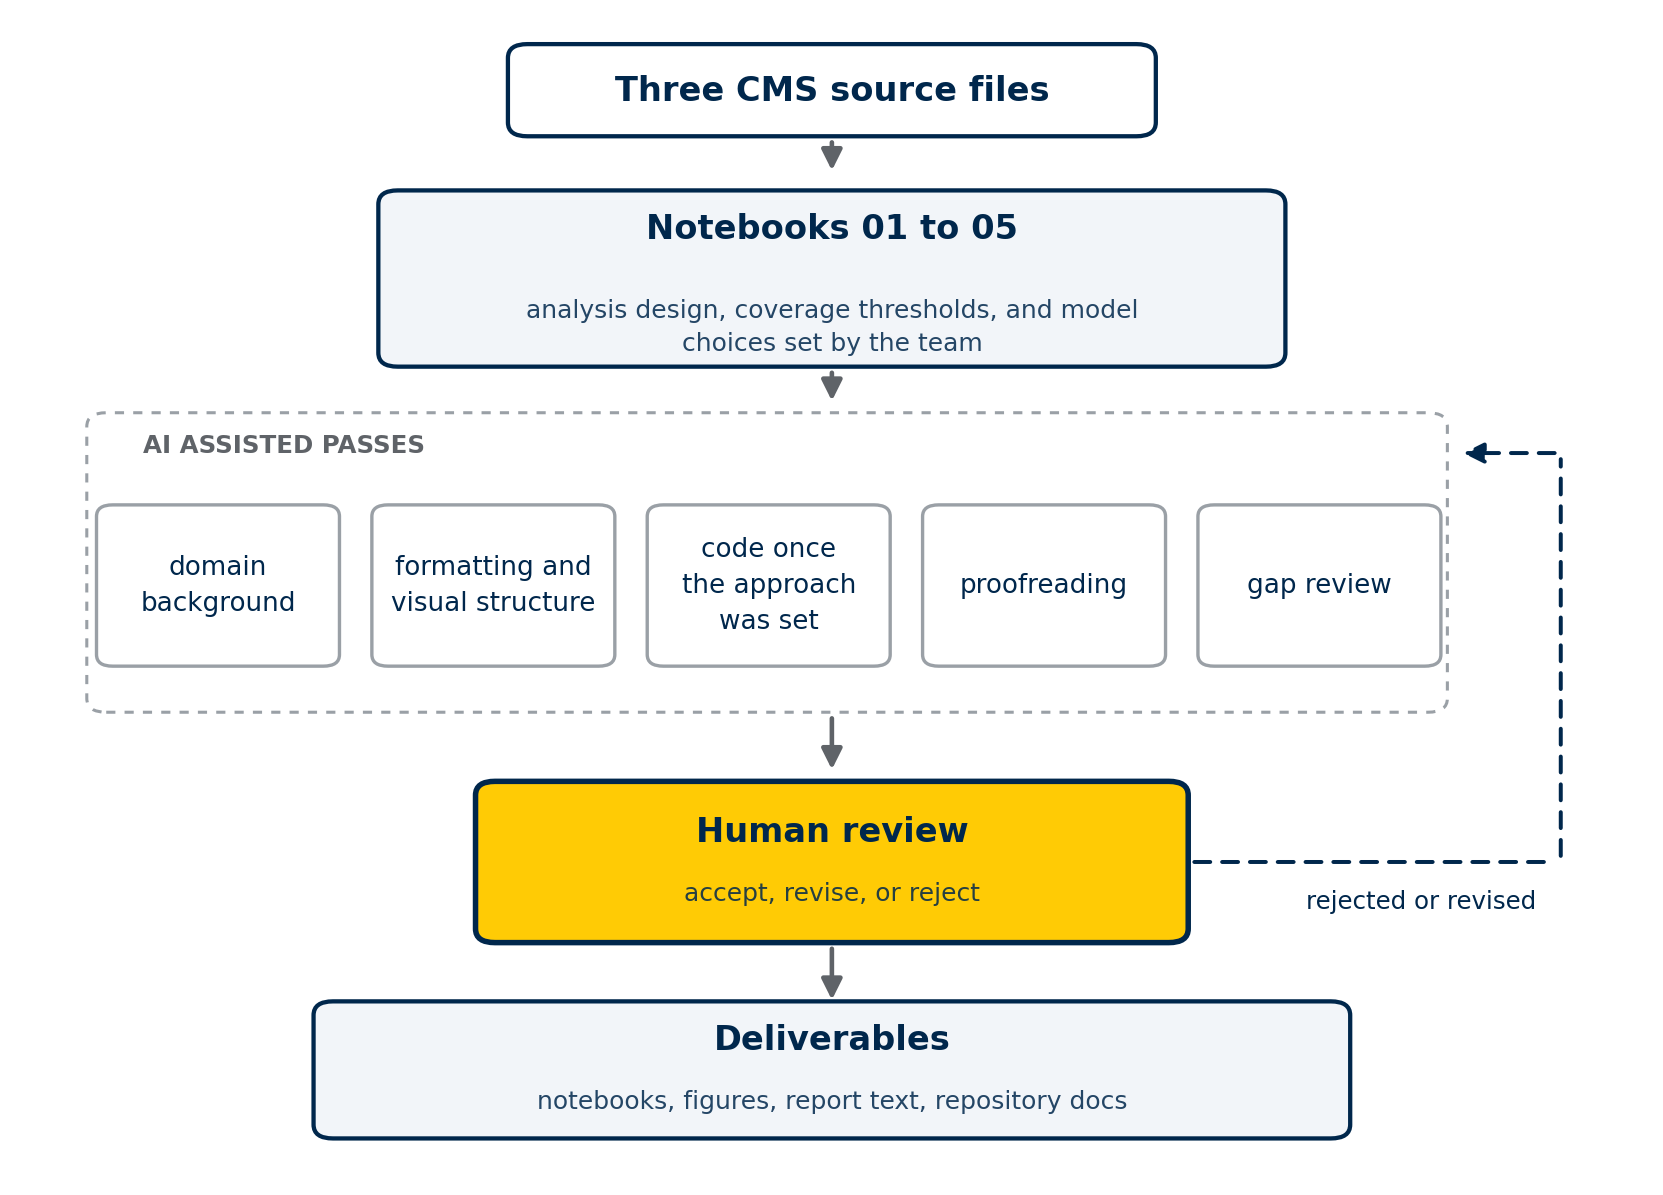
\includegraphics[width=0.95\textwidth]{figures/ai_workflow_chart.png}
    \caption{Diagram of AI workflow used in project.}
    \label{fig:ai_workflow}
\end{figure}

\subsection{Models and settings}

\begin{itemize}
    \item ChatGPT Codex Sol 5.6, run through Codex CLI 0.147.0 (data loading and review)
    \item Claude Code with Opus 4.8 (supervised learning)
    \item Cursor with Opus 4.8 (unsupervised learning)
\end{itemize}

Temperature is not configurable in Claude Code. Reasoning effort was set to high for review and medium for smaller tasks.

\subsection{Prompting and review}
We used AI either for a specific task or to challenge the analysis. Prompts pointed to the relevant notebook, figure, or result. One example of a prompt we used is as follows:

\begin{quote}
Can you play devil's advocate and review the analysis for methodological holes, weak assumptions, leakage, bias, or conclusions that may be overstated?
\end{quote}

AI suggestions were checked against the code and notebook outputs before being used.

One example of an evaluation we used is as follows: AI suggested quoting gradient boosting because it had the largest MIPS increment (+0.020). We checked fold-level results: that gain was positive in only two of five held-out states, so we revised the AI suggestion and reported Elastic Net instead (+0.017, positive in all five).

\newpage
\bibliography{references.bib}
% Context
\bibliographystyle{IEEEtran}

\end{document}
